\documentclass[a4paper,11pt]{article}
\usepackage[osf]{mathpazo}
\usepackage{ms}
\usepackage{natbib}
\usepackage{graphicx}
\usepackage{caption}
\usepackage{hyperref}
\usepackage[labelfont=bf]{caption} % make label for figure bold

% Allow referencing into the supporting information, once that exists.
\IfFileExists{./competition-kernels-sm.tex}{%
  \usepackage{xr}%
  \externaldocument{competition-kernels-sm}}{}

% We will generate all images so they have a width \maxwidth. This means
% that they will get their normal width if they fit onto the page, but
% are scaled down if they would overflow the MAPgins.
\makeatletter
\def\maxwidth{\ifdim\Gin@nat@width>\linewidth\linewidth\else\Gin@nat@width\fi}
\def\maxheight{\ifdim\Gin@nat@height>\textheight\textheight\else\Gin@nat@height\fi}
\makeatother
\setkeys{Gin}{width=\maxwidth,height=\maxheight,keepaspectratio}

\title{Trait gradients}

\author{ Georges Kunstler, Daniel S. Falster, Richard G. FitzJohn}
\date{}
\affiliation{Department of Biological Sciences, Macquarie University,
  Sydney, Australia}
\runninghead{}
\keywords{}

\usepackage{color}

\newcommand{\ud}{\ensuremath{\mathrm{d}}}
\newcommand{\sign}{\mathop{\mathrm{sign}}\nolimits}
\newcommand{\Rstar}{\ensuremath{R^*}}
\newcommand{\plant}{{\tt plant}}
\newcommand{\hmat}{\ensuremath{h_{\text{mat}}}}
\newcommand{\TODO}{{\color{red}\sc todo}}


\begin{document}

\mstitleshort
%\mstitlepage
\parindent=1.5em
\addtolength{\parskip}{.3em}

% \begin{abstract}
% Abstract goes here\ldots
% \end{abstract}

\section{Background \& Motivation}


NEED TO CLEAN UP THAT TO HAVE A FOCUS ON THEO MODEL!!

Understanding changes in vegetation composition across large biogeographic gradients is fundamental because vegetation is key to control ecosystem functioning, such as net primary production, and carbon storage. These changes in composition are also fundamental to understand biodiversity, as turnover in species composition explain a large proportion of the global diversity ($\beta$ diversity). In addition, these patterns are also the outcomes of long-term evolutionary adaptation. Understanding the drivers of these patterns is important not only for its intrinsic interest, but also as a path towards understanding how vegetation may change as result of environmental change.


\clearpage

\section{Potential mechanisms for these patterns}

Documenting empirical patterns of variation of plant traits along climatic gradient represents a key first step to understand changes in vegetation composition, but so far very few studies have proposed mechanisms to explain these traits patterns. These mechanisms need to explain the variation among sites with different climate but also the large variation within site resulting from the coexistence of interacting species with a range of trait values. A key element is thus that any mechanisms proposed need to account for the effect of the climate on the species traits but also on the effect of traits on species interaction and coexistence.

A promising approach for investigating causes of trait adaptation is via models capturing process of adaptation -- allow you to encode various rules and see how virtual system responds. Many abstract theoretical models, explored how species local climate adaptation, competitive interactions, and limited gene flow can drive species evolution and changes in traits composition along theoretical gradients \citep{Case-2000,Doebeli-2003,Goldberg-2006,Leimar-2008}. These studies generally showed that competition can limit species range and results in non continuous variation of traits value along the gradient. Most of abstract theoretical models are based on strong assumption about how traits are link to the competition and the response to the environmental gradient. Generally, one single traits determines both the local adaption to the abiotic conditions -- through the distance to an optimal trait value varying along the gradients -- and the competitive interaction -- through a normal competition kernel based on trait value of the species and its competitors\citep[see][]{Case-2000}.

The overall dominance of this classical view is surprising because other views about the link between traits and response to climate constrains and competition has been proposed in the literature. A common alternative view -- which can be traced back to Keddy's shifting competitive hierarchy \citep{Keddy-1989}-- proposes that all plant species have their physiological optima at the high productivity end of the gradient (low frost and drought stresses) but they differs in their tolerance to climate stresses and in term of their competitive abilities\citep{Keddy-1989}. Central to this view are the traits that underpin a tradeoff between species tolerance to climate stress \textit{vs.} their competitive abilities which shape species distributions along the gradient. Surprisingly, the number of theoretical models developed based on this alternative view of the effect of traits is extremely limited in comparison with the classical view \citep{Smith-1989,Lienard-2016}. These ideas has also been discussed around the idea of shift of the ranking of species carrying capacity \citep{Case-2005} and is connected to competition \textit{vs.} stress tolerance trade-off \citep{Muller-Landau-2010}, a variation of teh competition-colonization trade-off.

The figure \ref{fig:theointro} presents these two contrasting view of the species sorting using a simple LV model.

\begin{figure}[ht]
\centering
\includegraphics{../figures/resLV_2.pdf}
\caption{\textbf{Two alternative view about the how response to abiotic gradients and competition interact to drive species distribution.} Left column: where species have different physiological optimum along the abiotic gradient and interact via symmetric competition. Right column:  species have all their physiological optima at the high productivity end of the gradient (low frost and drought stresses)and interaction via asymmetric competition.
\label{fig:theointro}}
\end{figure}


One of the key reason that limit our progress on this question is that very few model start from the mechanisms of competition for resources and the physiology of the response to the environmental gradient to predict how traits will drive species joint response to climatic gradient and competition. Thus very few of these models are able to connect with real gradients,
real traits and the underlying physiological mechanisms. Several model
analyze how traits influence the physiological performance of single
plant in function of the local abiotic conditions \citep{Sterck-2011}
(\textbf{need to look also at optimisation cost-benefit models seek, ask Mark
and see other Sterck publications READ GIVNISH}) to explain how traits explain changes in individual performances along gradients. These \textit{physiological models} have been focused on effect of climate on growth, but much less is understood in term of effect on mortality or recruitment precluding our ability to translate these effects on population dynamics or community assembly. Recently a few studies have nevertheless started to extend this approach to whole community by including traits in DGVM models \citep[see][]{Sakschewski-2015,Scheiter-2013}. But they have been largely unsuccessful at explaining large-scale gradients probably mainly because we still lack clear understanding of the physiological mechanisms at play.
% We need to organise more clearly this section as optimisation model
% can also be viewed as adaptation model. The two mains points would
% be (i) model and their limitations and (ii) the observed gradients
% with higher variance within site than between sites and their lack
% of connection with model. The output would be to show that model need
% to be based on key physiological mechanism to allow connection with
% the field and that to deal with the large within site variance
% model need to include interplay between mechanisms allowing
% coexistence and abiotic effect. It may be also interesting to have
% few lines one abiotic filtering debate.

Here we propose to first compare theoretical prediction of a model based on the classical view \textit{vs.} a model based on the shifting competitive hierarchy.


\clearpage

\section{Theoretical Cellular Automaton of Competition vs. climate stress tolerance tradeoff}

It is surprising that so few theoretical models have been developed to test the alternative view on the link between traits and species response to the joint effect of climate gradient and competition.
Here we propose to explore these alternative building on the 'shifting competitive hierarchy' based on the few existing field studies that have documented such trade-off for tree. It seems that such tradeoff might occurs for two key dimension of tree competitive ability: tree competitive ability in early or in late successional stages. For instance \citep{Loehle-1998} proposed the existence of a tradeoff between tree maximum height growth – a key determinant of competitive ability in early successional stage – and frost tolerance, but this has been tested in only in two studies \citep{Koehler-2012,Savage-2013}. A few studies also explored trade-off between tree’ shade-tolerance -–a key component of competitive ability in late successional stage-- and frost tolerance \citep{Lusk-2013} or drought tolerance \citep[see][]{Smith-1989,Niinemets-2006} but see also \citep{Sack-2004,Markesteijn-2011}.


\subsection{Theoretical model description}

The model is implemented in Cpp vi RCpp in the following R package
TheoTradeOff \url{https://github.com/kunstler/TheoTradeOff}. The
model build on \citet{Pacala-1998} to represents the succession
dynamics but in cellular automaton rather than through
differential equation. We assume that species are defined by three
traits $c_e$, $c_l$, and $c_s$ describing
respectively their competitive ability in early and late successional stage and their
tolerance to abiotic stress.

The model describe a large meta-community structured in discrete cell
corresponding  to the  size of  an  adult individual.   The cells  are
connected  by local  dispersal  of  seed from  adults. Each adult
produces one seed per time step which is dispersed in the moore
neighborhood.  The cell  are structured along a  gradient of
abiotic stress. The meta-community is organized in rectangle of
256 x 256*N cells  and the abiotic stress  gradient run along the
largest side of the rectangle.

Individual are subject to two
types of mortality random perturbation controlled by
$prob_{distur}$ resulting in local extinction -which are  similar for all
species  and cells - and  abiotic stress  related mortality which
increased with the abiotic stress gradient (see below). Seed
establishment is controlled by the successional stage and
competitive interactions. For the successional dynamics, cells
are in one of three states: (1) empty thus in early successional
stage, (2) occupied but in early successional stage or (3)
occupied and in early successional stage. An occupied and early
successional stage has a given probability $prob_{suc}$ to
progress to late successional stage which control the speed of
succession. The probability of a seed establishing in a given
cell is function of the species already present in the cell and
is controlled by the hierarchy of their relevant competitive
ability (early or late successional stage). For instance the
probability of a seed of species $i$ to colonize a
early-successional cell occupied by the species $j$  is
controlled by their traits $c_{e,i}$ and $c_{e,j}$ by the
following equation \citep[as in][]{Law-1997}:

\begin{equation}
\label{eq:Law}
P(i \, win \, over \, j)=\left(\frac{1}{1+e^{-K(c_{e,i}-c_{e,j})}}\right).
\end{equation}

Where the parameter $K$ controls the asymmetry of the competition
\citep[see][]{Law-1997,Calcagno-2006}. The same apply in cells in
late-successional stage but with $c_l$. The species ability
mortality to tolerate abiotic stress is controlled by $c_s$, with
species with higher value of $c_s$ having a lower mortality rate
at a given level of stress $a$.

\begin{equation}
\label{eq:MortaStress}
P(morta | c_s , a)= (1- c_s) a
\end{equation}



   This trait textit{c]  is also
related  to  the  sensitivity  of  their  mortality  to  the  climatic
gradient.  Equations  1  describe  how  the probability  of  wining  a
competitive  event  is  influenced  by  the traits  of  the  different
species. Equation 2 describe how the mortality response to the climate
stress gradient is influenced by the trait \textit{c}.

Every time step, all cells of the rectangular landscape is updated by
1. testing  if the  individual in  the cell survive  or not  based on
disturbance, local climate  stress and it trait \textit{c},  and 2. by
testing  if the  neigboroud cells  disperse  seed in  the pacths  and
whether they  establish depending on the preemption  paramters and the
competitive interaction  between all seed  dispersed to the  cell. In
first step I will use local  dispersion in the 8 nearest cells (moore
neighborood). I need  to decide the best
solution  to describe  the  multi-species competition  event. A  first
solution  is to  compute the  probability of  every  pairs competitive
interaction and then average per  individual. There is however a exact
solution to this  that may save some computation  time. Need to search
in multinomial logistic regression.

\subsection{Triangular tradeoffs}

Species strategies are defined by the three traits $c_e$, $c_l$,
and $c_s$ which are constrained by a `triangluar` trade-off,
which impose that $c_e + c_l + c_s = 1$ (see figure \ref{fig:triangtrade}).

\begin{figure}[ht]
\centering
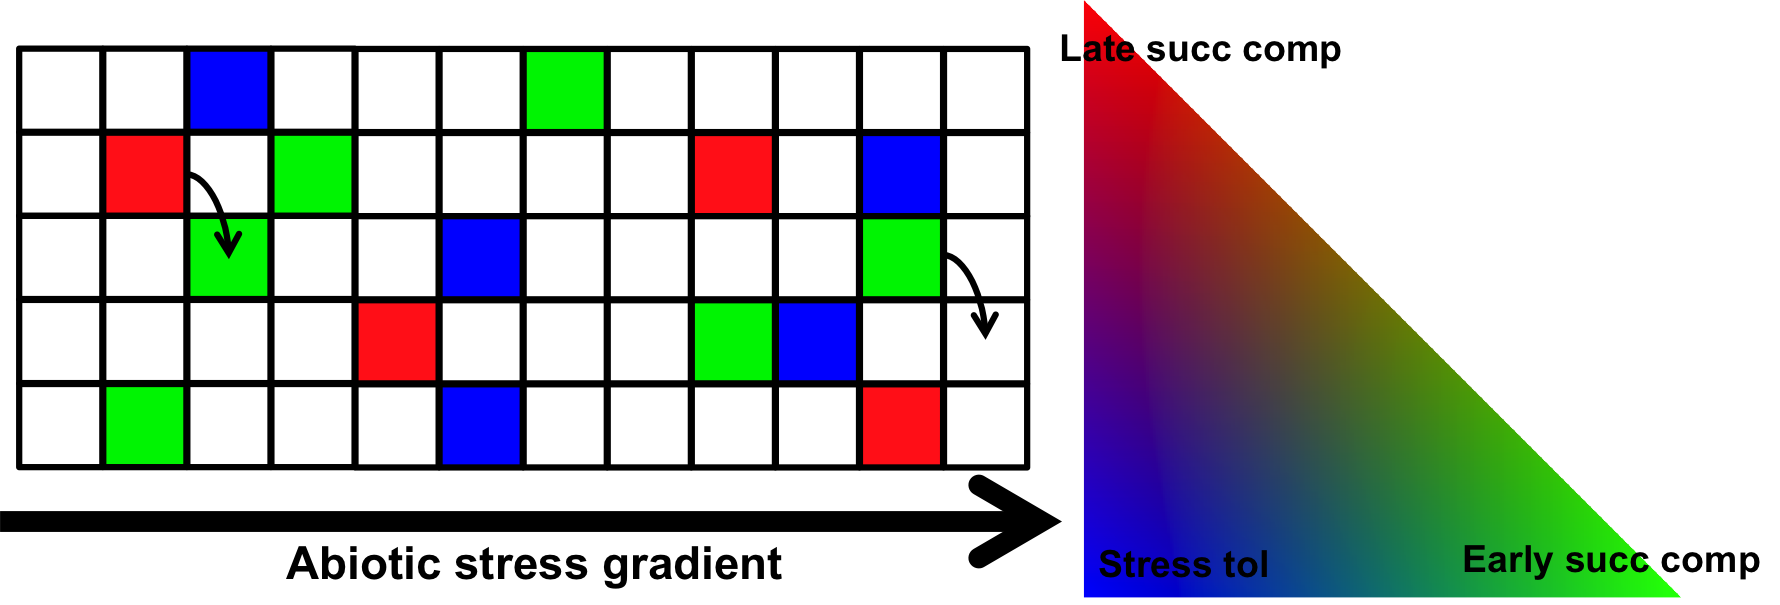
\includegraphics{../figures/auto.png}
\caption{\textbf{Cellular cellular automaton representing species
    dynamics along a rectangular landscape set along an abiotic
    gradient. Each cell is occupied by only one individual and
    dispersion is within the 8 neighboring cells. Species are
    defined by three traits defining a triangular tradeoff
    between early- or late-successional competitive ability
    \textit{vs.} climate stress tolerance.}
\label{fig:triangtrade}}
\end{figure}

\subsection{Results}

\begin{figure}[ht]
\centering
\includegraphics{../figures/map_theo_K100.pdf}
\caption{\textbf{Simulation of species distribution along a abiotic stress gradient.}
\label{fig:mapK100}}
\end{figure}


\clearpage


\bibliographystyle{amnat}
\bibliography{references}
\end{document}

%%  LocalWords:  LMA WD optimisation Falster successional LLS et
%%  LocalWords:  Glopnet stomatal Farquhar Poorter RGR Charrier
%%  LocalWords:  cavitation cavitated Skelton Isohydric Onoda al
%%  LocalWords:  anisohydric Niinemets Simova Laughlin Fortunel
%%  LocalWords:  Douma VanBodegom Kooyman rainforests
